\documentclass{llncs}
%
\usepackage[T1]{fontenc}
% T1 fonts will be used to generate the final print and online PDFs,
% so please use T1 fonts in your manuscript whenever possible.
% Other font encondings may result in incorrect characters.
%
\usepackage{graphicx}
% Used for displaying a sample figure. If possible, figure files should
% be included in EPS format.
%
% If you use the hyperref package, please uncomment the following two lines
% to display URLs in blue roman font according to Springer's eBook style:
%\usepackage{color}
%\renewcommand\UrlFont{\color{blue}\rmfamily}
%\urlstyle{rm}
%
\usepackage[spanish, es-noshorthands]{babel}
\addto\captionsspanish{\renewcommand{\tablename}{Tabla}} %Para que diga Tabla en vez de Cuadro
\usepackage{dsfont, amsmath}

\usepackage{caption}
\usepackage{subcaption}  % Para tener captions dentro de las subfiguras
\captionsetup{font=small}%para que las captions de las figuras sean más chicas

\usepackage{amssymb}
\usepackage{booktabs} % For better table formatting
\usepackage{graphicx} % Required for inserting images
\usepackage[colorlinks=true, urlcolor=blue, linkcolor=blue, citecolor=green]{hyperref}
%linkColor = citas internas cómo ref
\usepackage{tikz}
\usetikzlibrary{arrows.meta}
\usetikzlibrary{decorations.pathmorphing}
\usepackage{algorithm}
\usepackage{algpseudocode}
\usepackage{pgf} % For arithmetic operations in TikZ
\usepackage{comment}
\usepackage{booktabs}
\usepackage{url} %For writing paths
\usepackage[normalem]{ulem}
\usepackage{multirow}
\usepackage{placeins} % For removing strange spaces
\newcommand{\scc}[1]{{\color{red}#1}}


\usepackage[style=apa]{biblatex} % <- AGREGAR ESTA LÍNEA
\addbibresource{biblio.bib} % <- AGREGAR ESTA LÍNEA

\input{secciones/macros}

\tikzset{
	nodo/.style={
		shape=circle,
		draw=black,
		line width=1pt,   
		minimum size=7mm
	},
	arista/.style={
		line width=1pt,  
		-{Latex[length=3mm]}  
	},  
	mySnake/.style={
		decorate, 
		decoration={snake, amplitude=.4mm, segment length=4mm, post length=1mm}
	}
}

\raggedbottom % This so that not all pages have the same height. 

\begin{document}
%
% ENGLISH VERSION
\title{Contribution title}

%\titlerunning{Abbreviated paper title}
% If the paper title is too long for the running head, you can set
% an abbreviated paper title here
%
\author{First Author\inst{1}\orcidID{0000-1111-2222-3333} \and
Second Author\inst{2,3}\orcidID{1111-2222-3333-4444} \and
Third Author\inst{3}\orcidID{2222--3333-4444-5555}}
%
\authorrunning{F. Author et al.}
% First names are abbreviated in the running head.
% If there are more than two authors, 'et al.' is used.
%
\institute{Princeton University, Princeton NJ 08544, USA \and
Springer Heidelberg, Tiergartenstr. 17, 69121 Heidelberg, Germany
\email{lncs@springer.com}\\
\url{http://www.springer.com/gp/computer-science/lncs} \and
ABC Institute, Rupert-Karls-University Heidelberg, Heidelberg, Germany\\
\email{\{abc,lncs\}@uni-heidelberg.de}}
%
\maketitle              % typeset the header of the contribution
%
\begin{abstract}
The abstract should briefly summarize the contents of the paper in
150--250 words. This is the English version of the abstract that 
provides a comprehensive overview of the research conducted, 
the methodology used, and the main findings obtained.

% keywords in lowercase
\keywords{first keyword\and second keyword\and another keyword}
\end{abstract}

% SPANISH VERSION
% Clear the previous title info and set Spanish version

% Spanish title and abstract
\begin{center}
\vspace{1cm}
{\Large \bfseries\boldmath Título de la contribución}

\vspace{0.5cm}
\end{center}

\begin{abstract}
\noindent En este artículo se aborda el problema de la explicabilidad en modelos de aprendizaje automático mediante métodos de feature attribution.

En particular, se estudia una variante de los Shapley values conocida como Asymmetric Shapley Values (ASV), que permite incorporar conocimiento causal en la explicación de modelos de forma model-agnostic. A partir del análisis de su complejidad, se demuestra que el cálculo exacto de ASV es polinomial en modelos cuya distribución de entrada está representada por una red bayesiana del tipo Naive Bayes, en contraste con SHAP, que es \#P-hard aún en este caso restringido.

Con el objetivo de extender estos resultados a clases más generales de redes bayesianas, se introduce una noción de clases de equivalencia sobre los órdenes topológicos del grafo causal subyacente, lo cual permite reducir drásticamente el número de permutaciones necesarias para computar ASV. Se presenta un algoritmo polinomial en el número de clases para identificarlas, y se implementa un esquema de cómputo exacto de ASV basado en estas clases. Además, se propone un nuevo método para computar en tiempo polinomial la predicción esperada de un árbol de decisión, sobre una distribución dada por una red bayesiana arbitraria, permitiendo así evaluar el algoritmo desarrollado para el cómputo de ASV en estos modelos. 

Por último, se propone un algoritmo aproximado para calcular el ASV en familias de DAG's causales del tipo polytree. Para ello, se desarrolla un algoritmo de muestreo aleatorio de órdenes topológicos de polytrees. Estos resultados respaldan la viabilidad del enfoque propuesto en estructuras causales realistas, y se contrastan empíricamente con SHAP tanto en precisión como en eficiencia computacional.
\bigskip


\keywords{ explicabilidad, árboles de decisión, Asymmetric Shapley Values (ASV), Shap, polytrees, ordenes topológicos}
\end{abstract}


\vspace{0.5cm}
\setcounter{page}{1}

\section{Introducción}

In recent years, the capabilities of artificial intelligence models have grown rapidly, along with the complexity of their architectures. 
This progress has enabled the solution of tasks that once appeared unattainable, such as the use of language models to solve complex mathematical problems \parencite{frontierMath}. 
At the same time, current systems have reached scales far beyond those of a few years ago, both in terms of the number of parameters and structural complexity \parencite{EpochLargeScaleModels2024}. 
This lack of transparency is especially problematic in sensitive settings, such as medical diagnosis or high-stakes decision-making, where producing an accurate prediction is not enough: it is equally important to understand how that prediction was made. In response to this challenge, the field of Explainable Artificial Intelligence (XAI) has emerged \parencite{mersha2024explainable}, aiming to develop methods capable of making model decisions more interpretable.

Within the field of explainability, one of the most influential approaches is feature attribution, where each input variable is assigned a score reflecting its contribution to the prediction. 
In this line of work, SHAP is one of the most well-known methods \parencite{shapOriginalPaper}. It is based on the Shapley values, a concept originating in cooperative game theory \parencite{shapley1953value}. 
Intuitively, Shapley values provide a fair way to distribute the total value achieved by a coalition among its participants, according to their average marginal contribution when joining. 
Translated to machine learning, features play the role of players, and the value assigned to each feature aims to quantify its contribution to the model’s prediction for a given instance.

Despite its popularity, SHAP has important limitations. On the one hand, depending on the family of ML models under consideration and the underlying distribution of the data, the computation of the Shapley values can be tractable or not. For example,
it is well-known that for product distributions the complexity of computing these scores is equivalent to the complexity of computing the average 
value of the model \parencite{van2022tractability}. In particular, this implies that there exist efficient algorithms for the case where the models are given, for example, by decision trees or by restricted families of circuits \parencite{arenas2023complexity}, while the problem is intractable whenever the models are more expressive, as in the case of neural nets. 
For more general families of distributions the problem becomes much harder: for instance, when considering Naive Bayes distributions, the computation of this score is intractable already when considering trivial models that only depend on one feature \parencite{van2022tractability}.

On the other hand, there are also concerns about the quality of the explanations it produces. In particular, it is not always clear how to interpret, in the context of AI models, the axioms inherited from game theory, and several works point out that these explanations may fail to adequately capture relationships 
such as dependence, relevance, or causality between variables \parencite{fryer2021shapley, marques2023logic, huang2023inadequacy}. More generally, there is no absolute consensus on what should be considered an “explanation” in AI: many current techniques are pragmatic approximations to a much broader problem related to understanding, causality, and human interpretability \parencite{MILLER20191, lipton2017mythosmodelinterpretability}.

The Asymmetric Shapley Values (ASV from now on) are a proposal introduced by \cite{frye2019asymmetric} to overcome some of these limitations. This variant incorporates causal information into the computation of attribution scores by restricting attention to permutations of variables that respect a causal graph. 
In this way, instead of treating all features symmetrically, priority is given to the more fine-grained ones (in the sense that the information they provide is not present in the other variables). This can produce explanations that are more faithful to the data-generating process and can help better detect phenomena such as bias or discrimination. 
Moreover, although ASV was primarily proposed to improve explanatory quality, it naturally raises the question of whether this additional restriction may also provide computational benefits.

Therefore, in this paper we address the problem of efficiently computing the ASV scores, which was not explored thoroughly in previous literature. We will prove that for some families of models for which
computing the Shapley values is intractable there are still polynomial time algorithms for computing the ASV. Inspired by this initial result, we develop an algorithm to compute the ASV exactly in more general contexts
by exploiting the fact that many permutations of the features can be grouped in a unique equivalence class to simplify computations. Finally, we also propose a flexible approximation scheme that allows to approximate the ASV as long as it is possible to (1) Sample a topological order of the causal graph uniformly at random, and (2) Sample a data point with respect to the data distribution after conditioning a subset of the features to have specific values. We instantiate all these general algorithms with particular 
examples of causal graphs and machine learning models and show experimentally that they are efficient.


\section{Definiciones}

En esta sección introducimos las nociones formales que utilizaremos a lo largo del trabajo. Primero definimos los \textit{Shapley values} y su instanciación al problema de \textit{feature attribution}. Luego presentamos los \textit{Asymmetric Shapley Values} (ASV), que incorporan información estructural mediante un grafo causal. Finalmente, introducimos las redes bayesianas como modelo para la distribución de los datos y describimos las familias restringidas de redes que consideraremos en nuestros resultados.

\subsection{Shapley values y feature attribution}

Trabajaremos con clasificadores binarios y features binarias. Esta restricción simplifica la notación sin afectar las ideas centrales ni los algoritmos desarrollados, que pueden extenderse naturalmente a dominios finitos más generales.

Sea $X$ un conjunto finito de features. Una \emph{entidad} sobre $X$ es una función
\[
e:X\to\{0,1\},
\]
donde $e(x)$ representa el valor que la entidad $e$ toma en el feature $x$. Denotamos por $\entities(X)$ al conjunto de todas las entidades posibles sobre $X$, y asumimos dada una distribución de probabilidad $\Pr$ sobre $\entities(X)$. Un \emph{clasificador binario} es una función
\[
M:\entities(X)\to\{0,1\}.
\]

Dado un modelo $M$ y una entidad $e$, un \emph{feature attribution score} es una función
\[
\phi:X\to\mathbb{R},
\]
donde $\phi(x)$ mide la relevancia del feature $x$ respecto de la predicción $M(e)$.

Uno de los métodos de atribución más estudiados es \SHAPscore{} \cite{shapOriginalPaper}, basado en los \emph{Shapley values} \cite{shapley1953value}. En teoría de juegos cooperativos, los Shapley values describen cómo repartir el valor total obtenido por una coalición entre sus jugadores. Más precisamente, dado un conjunto finito de jugadores $\players$, una \emph{función característica} es una función
\[
\charactheristicFunction:\mathcal{P}(\players)\to\mathbb{R}
\]
que asigna un valor a cada coalición. Los Shapley values son la única asignación de pagos que satisface simultáneamente un conjunto de axiomas clásicos: \emph{eficiencia}, \emph{simetría}, \emph{jugador nulo} y \emph{linealidad}. Una forma cerrada de definirlos es la siguiente.

\begin{definition}[Shapley values]
	Sea $\players$ un conjunto finito y sea $\charactheristicFunction:\mathcal{P}(\players)\to\mathbb{R}$ una función característica. Para cada jugador $i\in \players$, su valor de Shapley se define como
	\begin{align}
		\phi_i(\charactheristicFunction)
		=
		\frac{1}{|\players|!}
		\sum_{\pi\in\perm(\players)}
		\left[
		\charactheristicFunction(\pi_{<i}\cup\{i\})-
		\charactheristicFunction(\pi_{<i})
		\right],
		\label{eq:shapley_values_by_perm_definitions}
	\end{align}
	donde $\perm(\players)$ es el conjunto de todas las permutaciones de $\players$, y $\pi_{<i}$ denota el conjunto de jugadores que aparecen antes que $i$ en la permutación $\pi$.
\end{definition}

Intuitivamente, esta expresión promedia la contribución marginal de un jugador sobre todos los órdenes posibles de llegada al juego. De manera equivalente, puede escribirse como
\[
\phi_i(\charactheristicFunction)
=
\sum_{S\subseteq \players\setminus\{i\}}
c_{|S|}
\left[
\charactheristicFunction(S\cup\{i\})-
\charactheristicFunction(S)
\right],
\]
donde
\[
c_m=\frac{m!(|\players|-m-1)!}{|\players|!}.
\]

En aprendizaje automático, el conjunto de jugadores se identifica con el conjunto de features $X$, en nuestro ejemplo de la red \cancerNetwork, $X$ sería el conjunto \variableNetwork{Cancer, Pollution, Dyspnoea, Xray}. Dada una entidad $e$ y un subconjunto $S\subseteq X$, queremos evaluar el comportamiento promedio del modelo al fijar los valores de las variables de $S$ según la entidad $e$ y marginalizar el resto de acuerdo con la distribución de los datos.

Para ello, definimos primero el conjunto de entidades \emph{consistentes} con $e$ en $S$:
\[
\consistsWith(e,S)=\{e'\in\entities(X): e'(x)=e(x)\text{ para todo }x\in S\}.
\]
La probabilidad condicionada a este conjunto queda dada por
\[
\Pr[e'\mid \consistsWith(e,S)] =
\begin{cases}
	\displaystyle
	\frac{\Pr[e']}{\sum\limits_{e''\in\consistsWith(e,S)} \Pr[e'']} & \text{si } e'\in\consistsWith(e,S),\\[1.2em]
	0 & \text{en caso contrario}.
\end{cases}
\]

Con esta notación, la función característica asociada a $M$, $e$ y $\Pr$ se define como la predicción promedio condicionada a los valores fijados en $S$.

\begin{definition}[Función característica inducida por un modelo]
	Dados un modelo $M$, una entidad $e$ y una distribución $\Pr$ sobre $\entities(X)$, definimos
	\begin{align}
		\charFunML_{M,e,\Pr}(S)
		=
		\sum_{e'\in\consistsWith(e,S)}
		\Pr[e'\mid\consistsWith(e,S)]\,M(e').
		\label{formula:characteristicFunctionDefinition_definitions}
	\end{align}
\end{definition}

Esto nos permite instanciar directamente los Shapley values en el problema de \textit{feature attribution}.

\begin{definition}[SHAP]
	Dado un modelo $M$, una entidad $e$, una distribución $\Pr$ y un feature $x_i\in X$, el valor SHAP de $x_i$ se define como
	\[
	\Shap_{M,e,\Pr}(x_i)
	=
	\sum_{S\subseteq X\setminus\{x_i\}}
	c_{|S|}
	\left[
	\charFunML_{M,e,\Pr}(S\cup\{x_i\})-
	\charFunML_{M,e,\Pr}(S)
	\right].
	\]
\end{definition}

Nótese que los axiomas que estos valores satisfacen no tienen un significado claro en el contexto de la inteligencia artificial, ya que dependen de la definición de \(\charFunML_{M,e,\Pr}\) \cite{fryer2021shapley}. Además, para algunas nociones simples y robustas de \textit{feature attribution} basadas en \textit{explicaciones abductivas} \cite{marques2023logic}, los Shapley values no logran asignar un puntaje de 0 a features irrelevantes \cite{huang2023inadequacy}. Aun así, constituyen uno de los marcos más influyentes para estudiar explicaciones locales basadas en atribución.

\subsection{Asymmetric Shapley Values y grafos causales}

La definición anterior trata a todas las permutaciones de features de manera uniforme. Sin embargo, en muchos problemas existe información estructural adicional que sugiere que no todos los órdenes son igualmente razonables. En particular, si se dispone de un grafo causal sobre las variables, resulta natural restringir la atención a aquellas permutaciones compatibles con dicha estructura.

La generalización más simple consiste en reemplazar el promedio uniforme por una función de pesos arbitraria sobre permutaciones.

\begin{definition}[Shapley values ponderados]
	Sea $w:\perm(\players)\to\mathbb{R}$ una función tal que $\sum_{\pi\in\perm(\players)} w(\pi)=1$. Definimos
	\begin{align}
		\phi_i^{assym}(\charactheristicFunction)
		=
		\sum_{\pi\in\perm(\players)}
		w(\pi)
		\left[
		\charactheristicFunction(\pi_{<i}\cup\{i\})-
		\charactheristicFunction(\pi_{<i})
		\right].
		\label{eq:assymetric_shap_def_definitions}
	\end{align}
\end{definition}

La familia de \emph{Asymmetric Shapley Values} propuesta en \cite{frye2019asymmetric} surge al elegir la función de pesos a partir de un DAG que codifica relaciones causales entre las features.

\begin{definition}[Asymmetric Shapley Values]
	Sea $G=(X,E)$ un DAG cuyos nodos son los features. Denotemos por $\topo(G)$ al conjunto de órdenes topológicos de $G$. Definimos la función de pesos
	\[
	w(\pi)=
	\begin{cases}
		\frac{1}{|\topo(G)|} & \text{si }\pi\in\topo(G),\\
		0 & \text{en otro caso}.
	\end{cases}
	\]
	Entonces, dado un modelo $M$, una entidad $e$ y una distribución $\Pr$, el valor ASV de un feature $x_i\in X$ se define como
	\[
	\assym_{M,e,\Pr}(x_i)
	=
	\frac{1}{|\topo(G)|}
	\sum_{\pi\in\topo(G)}
	\left[
	\charFunML_{M,e,\Pr}(\pi_{<i}\cup\{x_i\})-
	\charFunML_{M,e,\Pr}(\pi_{<i})
	\right].
	\]
\end{definition}

La intuición detrás de esta definición es que sólo se consideran órdenes que respetan la causalidad. De este modo, si una variable $x$ es causa de una variable $y$, entonces $x$ siempre aparece antes que $y$ en las permutaciones admitidas. Esto tiende a favorecer a las variables causalmente anteriores y a reducir la importancia de variables que son meramente consecuencias de otras. En consecuencia, ASV constituye una variante de SHAP diseñada para capturar asimetrías estructurales entre las features.

\subsection{Redes bayesianas como modelo de distribución}

Para evaluar las cantidades definidas arriba no alcanza con fijar un modelo predictivo: también es necesario especificar una distribución sobre el espacio de entidades. En este trabajo utilizamos redes bayesianas para representar dicha distribución.

\begin{definition}[Red bayesiana]
	Una Red Bayesiana $\aBayesianNetwork$ sobre un conjunto de variables $X$ es una tupla
	\[
	\aBayesianNetwork=(X,E,\Pr),
	\]
	donde $(X,E)$ es un DAG y, para cada variable $x\in X$, se especifica una distribución condicional
	\[
	\Pr(x\mid \parents(x)).
	\]
	Estas distribuciones se representan mediante tablas de probabilidad condicional (\emph{Conditional Probability Tables}, CPTs).
\end{definition}

La propiedad central de una red bayesiana es que factoriza la distribución conjunta usando únicamente dependencias locales. Si $X=\{X_1,\dots,X_n\}$, entonces
\[
\Pr(X_1,\dots,X_n)=\prod_{i=1}^n \Pr(X_i\mid \parents(X_i)).
\]
Esta factorización permite realizar inferencia probabilística de forma mucho más eficiente que manipulando directamente la distribución conjunta.

Conviene distinguir con cuidado entre \emph{red causal} y \emph{red bayesiana}. Una red bayesiana modela dependencias condicionales y define una distribución conjunta; un grafo causal, en cambio, pretende reflejar relaciones de causa y efecto entre variables. En general, ambas nociones no coinciden necesariamente. Sin embargo, en este trabajo asumiremos que el DAG subyacente a la red bayesiana puede utilizarse también como grafo causal para definir ASV. Esta decisión responde a dos motivos: por un lado, es consistente con el tipo de datos y experimentos que analizamos; por otro, nos permite estudiar simultáneamente el costo de la inferencia probabilística y el efecto de imponer restricciones causales en el cálculo de explicaciones.

Más precisamente, dado un modelo $M$, una entidad $e$ y una red bayesiana $\aBayesianNetwork$ sobre las features, utilizaremos la distribución inducida por $\aBayesianNetwork$ para calcular la función característica $\charFunML_{M,e,\Pr}$, y el DAG de $\aBayesianNetwork$ como estructura causal para definir $\assym_{M,e,\Pr}$.

\subsection{Familias restringidas de redes bayesianas}

La complejidad de la inferencia en redes bayesianas depende fuertemente de la estructura del grafo subyacente. En redes generales, calcular probabilidades marginales o condicionadas es un problema $\sharpPhard$, mientras que para ciertas familias restringidas la inferencia puede realizarse en tiempo polinomial. Por esta razón, nuestros resultados se concentran en clases estructurales bien delimitadas.

La primera familia que consideramos es la de las redes \emph{Naive Bayes}. En este caso, existe una variable raíz $X_1$ tal que todas las demás variables son sus hijas, y no hay otras aristas. Es decir, el conjunto de aristas es
\[
E=\{(X_1,X_j):2\leq j\leq n\}.
\]
La distribución conjunta factoriza entonces como
\[
\Pr[e]=\Pr[X_1=e(X_1)]\prod_{j=2}^n \Pr[X_j=e(X_j)\mid X_1=e(X_1)].
\]

\echu{Hace falta mostrar la fórmula de la probabilidad o mejor mostrar la imagen de que estructure tiene y listo? Igual la imagen ocupa espacio y no suma tanto, tal vez no hace falta ninguna de las dos.}
Esta familia es especialmente relevante porque, aunque su estructura es muy simple, ya permite exhibir una diferencia fundamental entre SHAP y ASV: se sabe que calcular SHAP sobre distribuciones Naive Bayes es intratable incluso para modelos muy simples \cite{van2022tractability}, mientras que uno de nuestros resultados muestra que ASV puede ser tratable en este escenario.

La segunda familia central en este trabajo es la de los \emph{polytrees}, es decir, DAGs cuyo grafo subyacente no dirigido es un árbol. Esta clase resulta importante porque admite inferencia probabilística en tiempo polinomial \cite{pearl1986bayesianInference}. Como el cálculo de la función característica involucra predicciones promedio condicionadas a evidencia, la posibilidad de realizar inferencia eficiente en la distribución de entrada es un ingrediente fundamental para obtener algoritmos tratables para ASV.

\echu{¿Se dice tratable o tractable?}

En síntesis, a lo largo de esta tesis trabajaremos principalmente con dos tipos de restricciones estructurales sobre la distribución de los datos: redes Naive Bayes, que sirven como caso base para nuestros resultados de tractabilidad, y polytrees, que constituyen la clase más general sobre la que desarrollamos algoritmos eficientes para inferencia y cómputo de explicaciones.

\section{Resultados teóricos}

\subsection{Tratabilidad de ASV}

Como vimos en la sección anterior, la complejidad de la distribución de entrada no es el único factor que determina la dificultad de calcular explicaciones basadas en Shapley values. De hecho, aun para distribuciones estructuralmente simples como las redes Naive Bayes, el cálculo exacto de SHAP sigue siendo intratable \cite{van2022tractability}. En contraste, los Asymmetric Shapley Values (ASV) restringen las permutaciones consideradas a aquellas compatibles con el grafo causal. En esta sección mostramos que esta restricción permite obtener tractabilidad en casos donde SHAP no la tiene.

\medskip

Consideramos el caso en que la distribución de los datos está dada por una red bayesiana Naive Bayes, y tomamos su DAG subyacente como grafo causal para calcular ASV. Recordemos que, en este caso, toda permutación topológica válida debe ubicar a la variable raíz $X_1$ antes que cualquier otra variable.

Esta observación permite caracterizar explícitamente el conjunto de órdenes topológicos y explotar la estructura de la distribución en el cálculo de ASV.

\begin{theorem}\label{the:asv_naive_bayes_tractable_clean}
	Sea $\mathcal{F}$ una familia de modelos. Los Asymmetric Shapley Values pueden calcularse en tiempo polinomial para distribuciones Naive Bayes si y solo si los Shapley values pueden calcularse en tiempo polinomial para $\mathcal{F}$ bajo distribuciones producto.
\end{theorem}

\echu{La demo es larga, la ponemos completa o damos una intuición la misma? Habría que ver el tema de si podemos mandar cosas al apéndice.}

\begin{proof}
	Primero, probamos la implicación de derecha a izquierda. Sea \(x_1\) el padre de todos los demás nodos en el DAG. Vamos a mostrar cómo calcular \(\assym_{M,e,\Pr}(x_j)\) para cualquier \(2 \leq j \leq n\) y \(\assym_{M,e,\Pr}(x_1)\) de forma independiente.
	
	Observemos que el DAG tiene \((n-1)!\) órdenes topológicos, uno para cada permutación de los features \(\{x_2, \ldots, x_n\}\), y \(\pi(x_1) = 1\) para todas ellas. Entonces,
	
	\[\label{eq:assymetric_for_naive_child}
	\assym_{M,e,\Pr}(X_j) = \sum_{\pi \in \topo(G)} w(\pi) \left[ \charactheristicFunction_{M,e,\Pr}(\pi_{<j} \cup \{x_j\}) 
	- \charactheristicFunction_{M,e,\Pr}(\pi_{<j}) \right]
	\]
	
	es equivalente a:
	
	\[
	\assym_{M,e,\Pr}(X_j) = \frac{1}{(n-1)!} \sum_{\pi \in \perm(\{x_2, \ldots, x_n\})} \left[ \charactheristicFunction_{M,e,\Pr}(\{x_1\} \cup \pi_{<j} \cup \{x_j\}) - \charactheristicFunction_{M,e,\Pr}(\{x_1\} \cup \pi_{<j}) \right]
	\]
	
	Así, una vez que \(x_1\) está fijado, la distribución para las variables \(x_2, \ldots, x_n\) es una distribución producto con \(p_{x_j} = P(X_j = 1 | X_1 = e(x_1))\). Para simplificar, asumamos que \(e(x_1) = 1\), y consideremos la distribución de producto \(\Pr'\) definida como:
	
	\[
	\Pr\,'[X_i = 1] = p_i = 
	\begin{cases}
		1 & i = 1 \\
		\Pr[X_i = 1 | X_1 = e(x_1)] & \text{en otro caso}
	\end{cases}
	\]
	
	que intuitivamente se obtiene de \(\Pr\) fijando \(X_1 = 1\). Siempre que \(x_1\) esté fijo, ambas distribuciones \(\Pr\) y \(\Pr'\) se comportan de la misma forma:
	
	
	\begin{lemma}\label{lemma:valuation_of_prob_function}
		Para cualquier \(S \subseteq X \setminus \{x_1\}\), se cumple que:
		\[
		\charFunML_{M,e,\Pr}(\{x_1\} \cup S) = \charFunML_{M,e,\Pr'}(\{x_1\} \cup S) = \charFunML_{M,e,\Pr'}(S)
		\]
	\end{lemma}
	
	\begin{proof}
		Esto se sigue de directamente manipulando la expresión:
		
		\begin{align}
			\charFunML_{M,e,\Pr}(\{x_1\} \cup S) &= \sum_{e' \in \consistsWith(e,\{x_1\} \cup S)} \Pr[e' | S] M(e') \nonumber \\
			&= \sum_{e' \in \consistsWith(e, \{x_1\} \cup S)} \left( \prod_{\substack{e'(y) = 1 \\ y \notin \{x_1\} \cup S}} p_y \prod_{\substack{e'(y) = 0 \\ y \notin \{x_1\} \cup S}} (1-p_y)\right) M(e')\\
			&= \sum_{e' \in \consistsWith(e, S)} \left( \prod_{\substack{e'(y) = 1 \\ y \notin S}} p_y \prod_{\substack{e'(y) = 0 \\ y \notin S}} (1-p_y)\right) M(e') \nonumber\\
			&= \sum_{e' \in \consistsWith(e, S)} \Pr\,'[e' | S] M(e') \nonumber\\
			&= \charFunML_{M,e,\Pr'}(S) \nonumber
		\end{align}
		
		donde la segunda igualdad viene de reemplazar $Pr$ por la distribución producto y la tercera igualdad se deduce al observar que para todas las entidades $e' \in \consistsWith(e, S)$ tales que $e'(x_1) = 0$ se cumple que 
		
		$$\prod_{\substack{e'(y) = 1 \\ y \notin S}} p_y \prod_{\substack{e'(y) = 0 \\ y \notin S}} (1-p_y) = 0$$
		
		Además, la segunda ecuación es igual a $\charFunML_{M,e,\Pr'}(\{x_1\} \cup S)$.
	\end{proof}
	
	
	%TODO: Seguir repasando esta demo y ver de entenderla bien de pi a pa
	Usando este lema, ahora demostramos
	
	\begin{align}\label{eq:relation_between_assym_and_shap_naive_child}
		\assym_{M,e,\Pr} (x_j) = \Shap_{M,e,\Pr'}(x_j)
	\end{align}
	
	Se cumple que %\sidesergio{Super menor, pero quizás en estas circunstancias siempre poner dos puntos:, o nunca}
	
	\begin{align*}
		\Shap_{M,e,\Pr'}(x_j) &= \frac{1}{n!} \sum_{\pi \in \perm(X)} \left[ \charFunML_{M,e,\Pr'}(\pi_{<j} \cup \{x_j\}) - \charFunML_{M,e,\Pr'}(\pi_{<j}) \right]\\
		&= \frac{1}{n!} \sum_{\pi \in \perm(X)} \left[ \charFunML_{M,e,\Pr'}(\{x_1\} \cup \pi_{<j} \cup \{x_j\}) - \charFunML_{M,e,\Pr'}(\{x_1\} \cup \pi_{<j}) \right]\\
		&= \frac{n}{n!} \sum_{\pi \in \perm(\{x_2,\ldots,x_n\})} \left[ \charFunML_{M,e,\Pr'}(\{x_1\} \cup \pi_{<j} \cup \{x_j\}) - \charFunML_{M,e,\Pr'}(\{x_1\} \cup \pi_{<j}) \right] \\
		&= \frac{1}{n-1!} \sum_{\pi \in \perm(\{x_2,\ldots,x_n\})} \left[ \charFunML_{M,e,\Pr}(\{x_1\} \cup \pi_{<j} \cup \{x_j\}) - \charFunML_{M,e,\Pr}(\{x_1\} \cup \pi_{<j}) \right]\\
		&= \assym_{M,e,\Pr}(x_j)
	\end{align*}
	
	donde la segunda y cuarta igualdad se siguen del Lema~\ref{lemma:valuation_of_prob_function}, la última igualdad de la Ecuación~\ref{eq:assymetric_for_naive_child} y la tercera al observar que para cada permutación de $\perm(\{x_2,\ldots,x_n\})$ podemos construir $n$ permutaciones de $\perm(X)$ insertando $x_1$ en todos los lugares posibles, y que para cada una de estas permutaciones la expresión dentro de la suma es la misma. Así, la Ecuación~\ref{eq:relation_between_assym_and_shap_naive_child} muestra que calcular $\assym_{M,e,\Pr}(x_j)$ se reduce a calcular los valores Shapley habituales para una distribución independiente particular.
	
	Ahora consideramos $\assym_{M,e,\Pr}(x_1)$. Observemos que
	
	\begin{align*}
		\assym_{M,e,\Pr}(x_1) &= \frac{1}{|\topo(G)|} \sum_{\pi \in \topo(G)} \left[ \charFunML_{M,e,\Pr}(\pi_{<1} \cup \{x_1\}) - \charFunML_{M,e,\Pr}(\pi_{<1}) \right]\\
		&= \frac{1}{|\topo(G)|}( \charFunML_{M,e,\Pr}(\{x_1\}) - \charFunML_{M,e,\Pr}(\emptyset))
	\end{align*}
	
	%\echu{¿En esta fórmula de Shap no falta el $\frac{1}{|\topo(G)|}$? Porque sino no se estaría normalizando el resultado.}
	
	ya que para todas las permutaciones el conjunto $\pi_{<1} = \emptyset$. Además, sabemos que $\charFunML_{M,e,\Pr}(\{x_1\}) = \charFunML_{M,e,\Pr'}(\emptyset)$ por el Lema~\ref{lemma:valuation_of_prob_function}, y que
	
	\begin{align*}
		\charFunML_{M,e,\Pr}(\emptyset) &= \sum_{e' \in \entities(X)} \Pr[e] M(e)\\
		&= \sum_{\substack{e' \in \entities(X) \
				\ e'(x_1) = 1}} \Pr[e' | e'(x_1) = 1] \Pr[X_1 = 1] M (e') + \sum_{\substack{e' \in \entities(X) \\ e'(x_1) = 0}} \Pr[e' | e'(x_1) = 1] \Pr[X_1 = 0] M (e')\\
		&= \Pr[X_1 = 1] \charFunML_{M,e,\Pr'}(\emptyset) + \Pr[X_1 = 0] \charFunML_{M,e,\Pr''}(\emptyset)
	\end{align*}
	
	donde la distribución $\Pr''$ es la distribución producto obtenida al fijar $X_1 = 0$ como
	
	\begin{align*}
		\Pr \, ''[X_i = 1] = \begin{cases}
			0 & i = 0\\
			Pr[X_i = 1 | X_1 = 0] & \text{de otro modo}
		\end{cases}
	\end{align*}
	
	Finalmente,
	
	\begin{align*}
		\assym_{M,e,\Pr}(x_1) = \frac{1}{|\topo(G)|}( (1 - \Pr[X_1 = 1]) \charFunML_{M,e,\Pr'}(\emptyset) - \Pr[X_1 = 0] \charFunML_{M,e,\Pr''}(\emptyset))
	\end{align*}
	
	y reducimos el problema de calcular $\assym_{M,e,\Pr}(x_1)$ al de calcular la predicción promedio del modelo $M$ para dos distribuciones independientes diferentes $\Pr'$ y $\Pr''$. Según \cite{van2022tractability}[Teorema 1], se cumple que estos promedios pueden ser calculados en tiempo polinomial si y sólo si los valores de Shapley pueden ser calculados en tiempo polinomial para una distribución de producto arbitraria.
	
	La demostración de izquierda a derecha sigue al observar que una distribución producto es un caso particular de una Distribución Naive Bayes en la cual, para cualquier valor del padre $X_1$, las distribuciones condicionales son las mismas.
	
	%\echu{ ¿Debería escribir la demo de izquierda a derecha? ¿O inecesario? No se si tiene mucho sentido, ya está muy pesada la tesis} Rta: No hace falta, con esto alcanza. 
	
\end{proof}

El Teorema~\ref{the:asv_naive_bayes_tractable_clean} muestra que, a diferencia de SHAP, ASV puede ser tratable al explotar la estructura causal. En particular, esta tratabilidad depende de poder calcular eficientemente la predicción promedio. En la experimentación nos enfocamos en árboles de decisión, donde desarrollamos algoritmos polinomiales para esta tarea.

\echu{Tiene sentido el teaser de la experimentación? O saco esa oración?}

\subsection{Clases de equivalencia y relación con los órdenes topológicos}

Recordemos la definición de ASV:
\[
\assym_{M,e,\Pr}(x_i)
=
\frac{1}{|\topo(G)|}
\sum_{\pi \in \topo(G)}
\left[
\charFunML_{M,e,\Pr}(\pi_{<i}\cup\{x_i\})-\charFunML_{M,e,\Pr}(\pi_{<i})
\right].
\]

Para simplificar la notación, en esta sección tomamos $M$, $e$ y $\Pr$ fijos, y escribimos simplemente $\charactheristicFunction$ en lugar de $\charFunML_{M,e,\Pr}$. La idea es reducir la cantidad de órdenes topológicos sobre los cuales evaluamos $\charactheristicFunction$, agrupando aquellos que devuelven el mismo resultado al evaluarse sobre $\charactheristicFunction$.

La relación ideal sería identificar dos órdenes topológicos $\pi^1,\pi^2 \in \topo(G)$ cuando
\[
\charactheristicFunction(\pi^1_{<i})=\charactheristicFunction(\pi^2_{<i}),
\]
pero esta condición es costosa de verificar, ya que requiere evaluar explícitamente la función característica. Por este motivo trabajamos con una relación más fina, puramente combinatoria.

\begin{definition}\label{def:equiv_relation_left_right}
	Sea $G=(V,E)$ un DAG y sea $x_i\in V$. Definimos la relación $\rel$ sobre $\topo(G)$ por
	\[
	\pi^1 \rel \pi^2
	\iff
	\{\pi^1_{<i}\}=\{\pi^2_{<i}\}.
	\]
	Es decir, dos órdenes topológicos son equivalentes si tienen exactamente el mismo conjunto de nodos a la izquierda de $x_i$.
\end{definition}

Esta relación depende únicamente de la posición relativa de los nodos respecto de $x_i$. Para representarla, resulta útil dividir los nodos del grafo en ancestros, descendientes y nodos no relacionados con $x_i$.

\begin{figure}[ht]
	\centering 
	\begin{tikzpicture}[scale=.95, transform shape]
		
		% ---- NODOS ----
		\node[nodo] (a1) at (0, 0) {$a_1$};
		\node[nodo] (a2) at (2.5, 2) {$a_2$};
		\node[nodo] (a3) at (2.5, -2) {$a_3$};
		\node[nodo] (xi) at (5, 0) {$x_i$};
		\node[nodo] (d_1) at (7.5, 2) {$d_1$};
		\node[nodo] (d_2) at (10, -2) {$d_2$};
		\node[nodo] (d_3) at (10, 0) {$d_3$};
		
		\node[draw=none, fill=none] (hijo_a3) at (3.5, -3) {};
		\node[draw=none, fill=none] (hijo_d2) at (9, -3) {};
		
		% ---- ARISTAS ----
		\path [->] (a1) edge[arista, mySnake]  (xi);
		\path [->] (a2) edge[arista, mySnake]  (xi);
		\path [->] (a3) edge[arista, mySnake]  (xi);
		\path [->] (xi) edge[arista, mySnake]  (d_1);
		\path [->] (xi) edge[arista, mySnake]  (d_2);
		\path [->] (xi) edge[arista, mySnake]  (d_3);
		\path [->] (a3) edge[arista, mySnake] node[above right] {} (hijo_a3);
		\path [->] (hijo_d2) edge[arista, mySnake] node[below right] {} (d_2);
		
	\end{tikzpicture}
	\caption{Al fijar un nodo $x_i$, dividimos el resto en tres grupos: ancestros ($a$), descendientes ($d$) y nodos no relacionados. Los ancestros siempre quedan a la izquierda de $x_i$, los descendientes siempre a la derecha, y solo los nodos no relacionados no tienen una posición fija respecto de $x_i$ entre distintos órdenes topológicos.}
	\label{fig:unrelatedNodesDefinition_paper}
\end{figure}

\begin{definition}\label{def:equivalence_class}
	Sea $G=(V,E)$ un DAG y $x_i\in V$. Una clase de equivalencia $\equivalenceClass$ queda determinada por una función
	\[
	f_{\pi}:V\setminus\{x_i\}\to \{\textit{left},\textit{right}\},
	\]
	donde $f_{\pi}(v)$ indica si el nodo $v$ aparece a la izquierda o a la derecha de $x_i$ en un orden topológico $\pi$. Denotamos por $L(\equivalenceClass)$ y $R(\equivalenceClass)$ a los conjuntos de nodos etiquetados con \textit{left} y \textit{right}, respectivamente.
\end{definition}

\begin{proposition}\label{prop:grouping_asv_by_eq_classes}
	Sea $eqCl(G,x_i)$ el conjunto de clases de equivalencia inducidas por $\rel$. Entonces
	\[
	\assym_{M,e,\Pr}(x_i)
	=
	\frac{1}{|\topo(G)|}
	\sum_{\equivalenceClass \in eqCl(G,x_i)}
	|\equivalenceClass|
	\left[
	\charactheristicFunction(L(\equivalenceClass)\cup\{x_i\})
	-
	\charactheristicFunction(L(\equivalenceClass))
	\right].
	\]
\end{proposition}

\begin{proof}
	Basta particionar la suma original de ASV por clases de equivalencia. Dentro de una misma clase, todos los órdenes topológicos inducen el mismo conjunto de nodos antes de $x_i$, y por lo tanto la expresión entre corchetes es constante.
\end{proof}

\echu{¿Es muy vende humo ponerle demostración? Sino lo escribo cómo un parrafo y le pongo que es la intuición.}

La ventaja de estas clases es que no requiere evaluar $\charactheristicFunction$ para decidir si dos órdenes pertenecen a la misma. La Proposición~\ref{prop:grouping_asv_by_eq_classes} muestra que, si podemos calcular eficientemente las clases de equivalencia y sus tamaños, entonces podemos computar ASV sin enumerar todos los órdenes topológicos.

\subsection{Algoritmo exacto para el cálculo de clases de equivalencia}
\label{alg:exact_algorithm_for_equivalence_classes}

Nuestro objetivo es computar $\assym_{M,e,\Pr}(x_i)$ dado un grafo causal $G$, el cual puede expresarse como una suma sobre clases de equivalencia de órdenes topológicos respecto de $x_i$. En consecuencia, el problema se reduce a calcular el conjunto $\eqClassSizes(G,x_i)$, es decir, las clases de equivalencia junto con sus tamaños.

\subsubsection{Enfoque naive}
\label{alg:naiveAlgorithmEquivalenceClass}

Un enfoque directo consiste en generar todos los órdenes topológicos de $G$ \cite{algorithmForAllTopoSorts} y luego agruparlos en clases de equivalencia según qué nodos no relacionados aparecen antes de $x_i$. A partir de esta agrupación, se obtiene un representante por clase y su tamaño.

Si bien este procedimiento es correcto, resulta computacionalmente ineficiente. En el peor caso, el número de órdenes topológicos crece factorialmente en el tamaño del grafo, es decir, $O(n!)$, lo cual vuelve impracticable este enfoque incluso para instancias moderadas. Esto motiva la necesidad de un algoritmo exacto que evite enumerar explícitamente todos los órdenes.

\subsubsection{Estructura del \textit{dtree} y estrategia general}

Proponemos un algoritmo recursivo que explota la estructura del \dtree{} inducido por el DAG alrededor del nodo $x_i$. Particionamos los nodos en tres conjuntos: ancestros $A$, descendientes $D$ y nodos no relacionados. Dentro de estos últimos, consideramos los subárboles cuyas raíces pertenecen al conjunto $UR$ (unrelated roots).

La idea central es descomponer el problema en dos etapas:
\begin{enumerate}
	\item calcular las clases de equivalencia de cada árbol no relacionado de manera independiente;
	\item combinar dichas clases con los ancestros y descendientes para obtener las clases completas.
\end{enumerate}

Cada clase de equivalencia se representa mediante una tupla
\[
(\equivalenceClassRep, leftTopos, rightTopos),
\]
donde $leftTopos$ y $rightTopos$ representan la cantidad de órdenes topológicos posibles a la izquierda y derecha de $x_i$, respectivamente. El tamaño de la clase es entonces $leftTopos \cdot rightTopos$.

La Figura~\ref{fig:ASV_forest_example} ilustra esta partición.

\begin{figure}[H]
	\centering
	\begin{tikzpicture}[scale=.65, transform shape, 
		unrelated/.style={circle, draw=red},
		ancestor/.style={circle, draw=blue},
		wiggly/.style={decorate, decoration={snake, amplitude=.2mm, segment length=2mm}}
		]
		\node[text=blue] at (-5, 0) {Ancestors};
		\node[text=teal] at (-5, -0.5) {Descendants};
		\node[text=red] at (-5, -1) {Unrelated};        
		
		\node[ancestor] (a1) at (0, 0) {$a_1$};
		\node[unrelated] (u1) at (-1, -2) {$u_1$};
		\node[ancestor] (a2) at (1, -2) {$a_2$};
		
		\drawUnrelatedTree{u2}{-1}{-4}{$u_2$}
		\node[ancestor] (a3) at (1, -4) {$a_3$};
		\node[unrelated] (u3) at (3, -4) {$u_3$};
		
		\drawUnrelatedTree{u4}{0}{-7}{$u_4$}
		\node[ancestor] (a4) at (3, -6) {$a_4$};
		
		\node[nodo] (xi) at (3, -8) {$x_i$};
		
		\drawUnrelatedTree{r1}{6}{0}{$u_5$} 
		\drawUnrelatedTree{r2}{10}{0}{$u_6$} 
		
		\node[draw=none, fill=none] (hi) at (3, -10) {};
		
		\path [->] (a1) edge (u1);
		\path [->] (a1) edge (a2);
		\path [->] (a2) edge (u2);
		\path [->] (a2) edge (a3);
		\path [->] (a2) edge (u3);
		\path [->] (a3) edge (u4);
		\path [->] (a3) edge (a4);
		\path [->] (a4) edge (xi);      
		\path [->, teal] (xi) edge[decorate, decoration={snake}] (hi);
	\end{tikzpicture}
	\caption{Partición del grafo en ancestros, descendientes y árboles no relacionados respecto de $x_i$.}
	\label{fig:ASV_forest_example}
\end{figure}

\subsubsection{Clases de equivalencia de árboles no relacionados}

Sea $UR$ el conjunto de raíces de árboles no relacionados. Para cada $ur \in UR$, calculamos recursivamente sus clases de equivalencia mediante la función $\unrEqCl$.

El caso base ocurre cuando $n$ es una hoja:
\[
\unrEqCl(n)=\{(\{n_l\},1,1),(\{n_r\},1,1)\}.
\]

Para un nodo interno, combinamos las clases de equivalencia de sus hijos y consideramos dos posibilidades: ubicar $n$ a la izquierda o a la derecha de $x_i$. Esto da lugar a la siguiente recurrencia:

\begin{align}
	\unrEqCl(n) = 
	\begin{cases} 
		\{(\{n_l\},1,1),(\{n_r\},1,1)\} & \text{si $n$ es hoja} \\[1ex]
		\bigcup_{\forall mix} \union(mix,n_{left}) \;\cup\; \union(right,n_{right}) & \text{en otro caso}
	\end{cases}
\end{align}

Existe una correspondencia biyectiva entre las clases de equivalencia de un nodo y las combinaciones de clases de sus hijos, lo cual garantiza la correctitud del esquema recursivo.

\subsubsection{Combinación con descendientes}

Los descendientes de $x_i$ siempre aparecen a la derecha, por lo que pueden tratarse como un bloque independiente. El número de órdenes topológicos de un \dtree{} enraizado en $n$ está dado por:

\begin{align}
	topoSorts(n)=
	\binom{\sum_{j} |T_{n_j}|}{|T_{n_1}|,\dots,|T_{n_{|n|}}|}
	\prod_{j} topoSorts(n_j),
\end{align}

lo cual refleja la intercalación de los órdenes de los subárboles hijos.

\subsubsection{Combinación con ancestros}

\echu{¿Debería explicar un poco menos en esta sección y meter menos fórmulas? La puedo escribir más por arriba.}

A diferencia de los descendientes, los ancestros imponen restricciones de precedencia. No es posible intercalar libremente nodos no relacionados con ancestros mediante coeficientes multinomiales.

Para resolver este problema definimos la función $leftOrders$, que contabiliza cuántas formas válidas existen de intercalar los nodos no relacionados (ubicados a la izquierda) con los ancestros, respetando las dependencias del DAG.

La Figura~\ref{fig:order_of_ancestors} ilustra una posible disposición de los ancestros.

\begin{figure}[ht]
	\centering
	\begin{tikzpicture}
		\draw[thick] (0,0) -- (10,0);
		\foreach \x/\label in {2/$a_1$, 4/$a_2$, 6/$a_3$, 8/$a_4$} {
			\node at (\x-1,0.2) {$\cdots$};
			\draw (\x,0.2) -- (\x,-0.2);
			\node[below] at (\x,-0.2) {\label};
		};
		\node at (9,0.2) {$\cdots$};
	\end{tikzpicture}
	\caption{Orden relativo de los ancestros.}
	\label{fig:order_of_ancestors}
\end{figure}

\begin{algorithm}
	\caption{leftOrders}
	\begin{enumerate}
		\item Determinar la posición del siguiente ancestro.
		\item Elegir nodos disponibles para ubicar antes de dicha posición.
		\item Actualizar el conjunto de nodos restantes.
		\item Continuar recursivamente.
	\end{enumerate}
\end{algorithm}

\subsubsection{Fórmula final}

Integrando ambos componentes, obtenemos que el conjunto completo de clases de equivalencia puede construirse a partir del producto cartesiano de las clases de equivalencia de los árboles no relacionados. Formalmente,

\begin{align}
	\eqClassSizes(G, x_i) = 
	\bigcup_{\forall mix \in \unrEqCl(ur_1)\times\dots\times\unrEqCl(ur_{|UR|})}
	\left(eqCl(A,D,mix),\eqClassSize(A,D,mix)\right).
\end{align}

Aquí, cada $mix$ representa una elección de clases de equivalencia para cada árbol no relacionado. A partir de dicha elección, la función $eqCl(A,D,mix)$ construye la representación completa de la clase, mientras que $\eqClassSize(A,D,mix)$ calcula su tamaño combinando:

\begin{itemize}
	\item la cantidad de intercalaciones válidas con los ancestros, dada por $leftOrders$;
	\item la cantidad de órdenes topológicos de los descendientes;
	\item y las contribuciones internas de los árboles no relacionados.
\end{itemize}

De este modo, la expresión anterior no solo enumera todas las clases de equivalencia, sino que también computa exactamente su cardinalidad, sin necesidad de generar explícitamente los órdenes topológicos.

\subsubsection{Complejidad}

La complejidad total del algoritmo está dominada por dos componentes principales:

\begin{itemize}
	\item el cálculo de $\unrEqCl$, que recorre recursivamente los árboles no relacionados y combina las clases de sus hijos;
	\item la combinación global de clases, que requiere procesar el producto cartesiano de dichas clases y, para cada combinación, computar $leftOrders$ y las contribuciones de los descendientes.
\end{itemize}

En consecuencia, el costo total puede expresarse como proporcional al número de combinaciones de clases de equivalencia generadas, multiplicado por el costo de combinarlas con ancestros y descendientes. En particular, si denotamos por $k$ el número total de clases de equivalencia resultantes, el algoritmo tiene complejidad del orden de $O(k^3 \cdot \text{poly}(n))$.

Si bien $k$ puede ser exponencial en el peor caso, este enfoque evita depender del número total de órdenes topológicos del grafo, que puede ser factorial. Por lo tanto, el algoritmo representa una mejora sustancial respecto del enfoque naive, especialmente en grafos donde el número de clases de equivalencia es significativamente menor que el número de órdenes topológicos.

\subsection{Aproximación de ASV mediante sampleo}

En las secciones anteriores nos concentramos en algoritmos exactos para calcular $ASV$, ya sea enumerando todas las clases de equivalencia o explotando su estructura para reducir la cantidad de evaluaciones de la función característica. Sin embargo, cuando el número de clases o de órdenes topológicos es demasiado grande, incluso estos enfoques pueden volverse prohibitivamente costosos. Esto motiva la consideración de algoritmos aproximados basados en técnicas de muestreo.

Siguiendo la idea de las clases de equivalencia, proponemos reemplazar la suma exacta que define $ASV$ por un promedio empírico sobre una muestra aleatoria. Este enfoque permite estimar el valor de $ASV$ con buena precisión utilizando una cantidad moderada de muestras, ya que el error del estimador decrece con el tamaño de la muestra.

Existen dos variantes naturales de esta estrategia. La primera consiste en samplear órdenes topológicos del DAG causal $G$ y estimar el valor de $ASV$ a partir de sus contribuciones marginales. La segunda consiste en samplear clases de equivalencia y utilizar un representante de cada clase para aproximar el promedio exacto.

En ambos casos, el punto central es disponer de un mecanismo que permita generar muestras con la distribución correcta (uniforme en el caso de órdenes topológicos, o proporcional al tamaño en el caso de clases de equivalencia). Bajo esta condición, el cálculo de $ASV$ se reduce a promediar evaluaciones de la función característica sobre muestras i.i.d.

Una ventaja fundamental de este enfoque es que desacopla el cálculo de $ASV$ de la estructura específica del grafo. En particular, mientras que los algoritmos exactos desarrollados anteriormente explotan propiedades estructurales como la de los \dtrees{} o polytrees, el enfoque basado en sampleo puede aplicarse a \emph{cualquier} DAG, siempre que se disponga de un procedimiento para generar muestras adecuadas. Esto amplía significativamente el alcance práctico del método.

El caso de órdenes topológicos resulta especialmente natural, ya que
\[
\assym_{M,e,\Pr}(x_i)
=
\frac{1}{|\topo(G)|}
\sum_{\pi \in \topo(G)}
\left[
\charFunML_{M,e,\Pr}(\pi_{<i}\cup\{x_i\})
-
\charFunML_{M,e,\Pr}(\pi_{<i})
\right]
\]
puede interpretarse como el valor esperado de la variable aleatoria
\[
Z_\pi =
\charFunML_{M,e,\Pr}(\pi_{<i}\cup\{x_i\})
-
\charFunML_{M,e,\Pr}(\pi_{<i}),
\qquad \pi \sim \mathrm{Unif}(\topo(G)).
\]
Por lo tanto, si podemos samplear órdenes topológicos uniformemente, obtenemos un estimador insesgado de $ASV$ promediando copias i.i.d.\ de $Z_\pi$. Además al tener algoritmos de sampleo de órdenes topologicos para DAGs en general y no solo \dtrees este algoritmo logra ser más general. 

También a partir de estos órdenes sampleados podemos dividirlos por sus clases de equivalencia al igual que el algoritmo naive con probabilidad proporcional a su tamaño y estimar el valor mediante el promedio de sus representantes. Veamos a continuación dos posibles estrategias de sampleo. 

\subsubsection{Sampleo uniforme de órdenes topológicos}
\label{subsubsection:toposort_sampling}

Nos concentramos en el problema de samplear órdenes topológicos de un DAG de manera uniforme. Un primer enfoque consiste en generar todos los órdenes topológicos mediante un algoritmo determinístico, como el de Knuth \cite{algorithmForAllTopoSorts}, y devolverlos a medida que se producen. Sin embargo, este procedimiento no resulta adecuado para sampleo: al ser determinístico, no genera una distribución uniforme y puede sesgar la muestra cuando distintos nodos fuente aparecen con frecuencias muy diferentes como comienzo de un orden.

La idea correcta consiste en construir el orden de manera recursiva. Sea $S$ el conjunto de nodos fuente de un DAG $D$. Para cada $s \in S$, definimos
\[
p(s)=\frac{\#\topo(D-\{s\})}{\#\topo(D)},
\]
donde $\#\topo(D-\{s\})$ es la cantidad de órdenes topológicos que comienzan con $s$. El algoritmo selecciona el primer nodo del orden según esta distribución y luego continúa recursivamente sobre el grafo restante.

Este procedimiento garantiza que los órdenes topológicos se generan con la distribución uniforme deseada, siempre que se disponga de un método para contar la cantidad de órdenes de los subgrafos. En nuestro caso, esto se logra mediante el algoritmo de conteo desarrollado previamente para polytrees.

\echu{¿Agrego la imagen para ilustrar este algoritmo o al pedo? Me parece que no porque no le deberíamos dar mucha bola, no es tan relevante.}

Aún así, el problema que tiene este algoritmo es que solo funciona para el caso de polytrees, y sabemos que además el conteo en DAGs generales es \sharpPhard, por lo que buscamos otra estrategía de sampleo distinta.

\echu{Agregar acá lo del algoritmo de sampleo para el caso general, acá tendría que implementarlo y contar que hicimos un experimento para ver cuál era mejor para el caso de un polytree, así comparamos los tiempos. }

\subsubsection{Error del sampleo}

El esquema de aproximación basado en sampleo depende de dos subrutinas: la capacidad de generar muestras y la de evaluar la función característica sobre cada una de ellas. En particular, el algoritmo consiste en samplear independientemente órdenes topológicos y promediar sus contribuciones marginales.

Más precisamente, si $\pi^{(1)},\dots,\pi^{(m)}$ son órdenes topológicos sampleados uniformemente, el estimador viene dado por
\[
\widehat{ASV}
=
\frac{1}{m}\sum_{j=1}^{m}
\left[
\charFunML_{M,e,\Pr}(\pi^{(j)}_{<i}\cup\{x_i\})
-
\charFunML_{M,e,\Pr}(\pi^{(j)}_{<i})
\right].
\]

Cada muestra requiere generar un orden topológico y evaluar la función característica una cantidad constante de veces. La cantidad de muestras necesarias para obtener una buena aproximación depende de la precisión deseada y puede acotarse mediante resultados estándar de concentración, como se detalla en el apéndice.

\echu{¿Hay apéndice? Si no hay apéndice, meto las demostraciones que tenemos sobre la estimación del error promedio acá? } 

De manera análoga, este enfoque puede aplicarse utilizando clases de equivalencia en lugar de órdenes topológicos, siempre que se puedan samplear con la distribución adecuada.

\echu{Queda medio raro meter esta sección acá, tal vez extraería la parte de la predicción promedio en una sección más y luego metería esto al final para poner algo de la experimentación. }

\subsection{Instanciaciones particulares}
\label{section:particular_instances}

En nuestro caso, nos enfocamos en árboles de decisión como modelo $M$, y en distribuciones $\Pr$ representadas mediante redes bayesianas. En este contexto, desarrollamos un algoritmo para calcular
\[
\charFunML_{M,e,\Pr}(S)
\]
basado en recorrer el árbol de decisión y acumular las condiciones de camino inducidas por cada rama. Para cada hoja compatible con la evidencia, se computa su probabilidad mediante inferencia en la red bayesiana y se pondera por la predicción de la hoja. La predicción promedio se obtiene sumando estos aportes.

Cuando la red bayesiana tiene estructura de polytree, la inferencia puede realizarse en tiempo polinomial, por lo que el costo de evaluar la función característica es también polinomial.

Esto induce un esquema general para calcular $ASV$: siempre que el sampleo/generación exacta de órdenes topológicos o clases de equivalencia sea eficiente, se obtiene un algoritmo aproximado cuyo costo total es polinomial en el tamaño de la instancia y en los parámetros de precisión.

Por el contrario, cuando la predicción promedio no puede calcularse eficientemente, este enfoque deja de ser aplicable. En particular, el Teorema~\ref{the:asv_naive_bayes_tractable_clean} sugiere que la tratabilidad de $ASV$ está intrínsecamente ligada al costo de computar dichas esperanzas, ya que cada muestra requiere evaluar una contribución marginal.

En síntesis, los algoritmos propuestos resultan especialmente efectivos en escenarios donde:
\begin{enumerate}
	\item el sampleo/conteo puede realizarse eficientemente;
	\item la predicción promedio es computable en tiempo polinomial;
	\item el número de órdenes o clases es demasiado grande para un enfoque exacto.
\end{enumerate}

Este es precisamente el régimen considerado en la experimentación.

\echu{Acá no mostre nada de la experimentación que queríamos contar en teoría, siento que para el flow debería venir acá. ¿Que experimentos metemos? Yo banco "Clases de equivalencia vs Órdenes Topológicos" y "ASV exacto sin EqClasses vs ASV aproximado"}

\subsection{ASV exacto}

Recordemos la fórmula introducida en la sección \ref{Section:HeuristicaASV} para ASV, utilizando nuestra heurística.

\begin{align*}
	\phi_{i}^{assym}(\charactheristicFunction) = \sum_{\pi \in \perm(\players)} w(\pi) \left[ \charactheristicFunction(\pi_{<i} \cup {i}) - \charactheristicFunction(\pi_{<i}) \right] &= \\
	\heuristicASVFormula
\end{align*}

Dado un DAG $G$, un nodo $x_i \in V(G)$ y una función característica $\charactheristicFunction$. Nuestro algoritmo completo queda así entonces: 

\begin{itemize}
	\item Calculamos $eqClass$ a través de $\eqClassSizes(G,x_i)$, el algoritmo que introducimos en la sección~ \ref{alg:exact_algorithm_for_equivalence_classes}
	\item Luego para cada clase de equivalencia vamos a calcular el promedio teniendo en cuenta los features previos a $x_i$. Para realizar el promedio vamos a utilizar el algoritmo de la sección \ref{section:particular_instances}. (En el caso de que el modelo no sea un árbol, podemos aproximarlo utilizando Monte Carlo u otro método)
	\item Por último sumamos los resultados para obtener él $\assym$ para el feature $i$. 
\end{itemize}

Las modificaciones que introducimos son para mejorar la performance del mismo, sin modificar los resultados obtenidos a diferencia del enfoque aproximado. En la sección a continuación vamos a ver cuál es la mejora respecto al enfoque naive y el tiempo que tarda para distintas redes.  

\subsection{ASV aproximado}

Este algoritmo es igual al anterior. La única diferencia que tiene es respecto a cómo se calculan las clases de equivalencia, $eqClass(G, x_i)$, puesto que ahora las vamos a aproximar. Además, vamos a tener que agregar un parámetro extra, para definir la cantidad de órdenes topológicos que queremos generar. 
Primero utilizamos los algoritmos vistos en \ref{subsubsection:toposort_sampling} para samplear los órdenes topológicos. Esto nos va a permitir calcular él $ASV$ para polytrees o DAGs y no simplemente \dtrees. Luego procesamos estos órdenes al igual que en la sección \ref{alg:naiveAlgorithmEquivalenceClass}, para obtener las clases de equivalencia. Una vez obtenidas las clases de equivalencia, repetimos el mismo proceso del algoritmo exacto. 


\section{Experimental results}

We evaluate the proposed methods by comparing them against naive baselines in terms of computational cost and scalability. 
Experiments were conducted on two real Bayesian networks, \cancerNetwork{} and \childNetwork{}, obtained from the \texttt{bnlearn} repository. Both were used as data distributions and as causal DAGs. The \childNetwork{} network was modified into a polytree by removing edges that introduce cycles in the underlying undirected graph.
Datasets were generated by sampling from these networks, and decision trees were trained accordingly. For ASV computation, the prediction variable was removed from the network to avoid trivial inference. To analyze the performance of the algorithms that compute the equivalence classes of topological sorts we also created artificial networks shaped as (1) Balanced binary trees, (2) Naive-bayes distributions, and (3) Trees composed by merging directed paths on their root (what we call \texttt{multiplePaths}).\footnote{All experiments were run on an Intel i5-7500 CPU @ 3.40GHz with 16 GB of RAM, using Ubuntu 22.04 and Python 3.12. The main libraries used were \texttt{pgmpy}, \texttt{sklearn}, \texttt{networkx}, and \texttt{shap}.}

\vspace{-3mm}

\paragraph{Equivalence Classes vs. Topological Orders} We compare the naive ASV computation based on iteratingg all topological orders with our approach based on equivalence classes. The key quantities are the sizes of $\topo(G)$ and $\Lambda^x_{G}$, as well as the cost of constructing each set.

\begin{figure}[ht]
	\centering
	\begin{subfigure}[b]{0.49\linewidth}
		\centering
		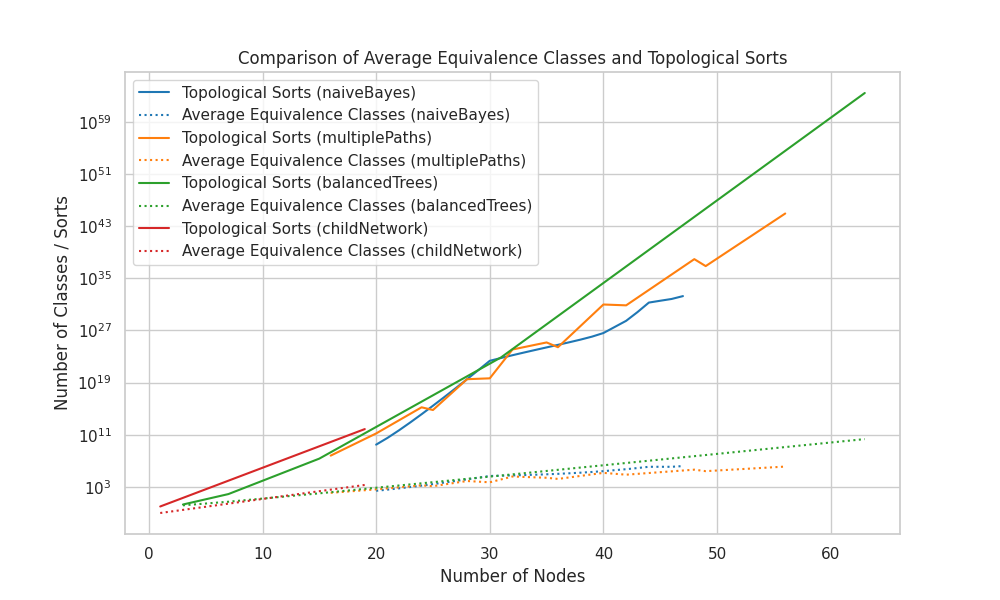
\includegraphics[width=\linewidth]{img/equivalentClassesVsToposorts.png}
		\caption{Number of equivalence classes vs. topological orders.}
		\label{fig:equivalenceClassesVsToposortsNumberPlot}
	\end{subfigure}
	\hfill
	\begin{subfigure}[b]{0.49\linewidth}
		\centering
		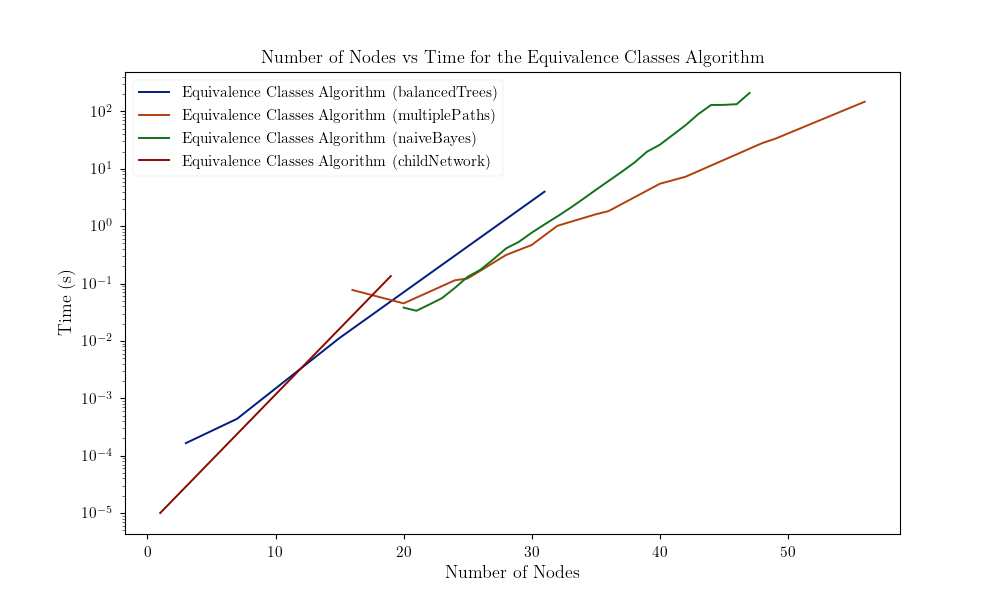
\includegraphics[width=\linewidth]{img/equivalentClasses_timevsNodes.png}
		\caption{Runtime for computing equivalence classes.}
		\label{fig:equivalenceClassesTimePlot}
	\end{subfigure}
	\label{fig:eq_vs_topo_combined}
\end{figure}

Figure~\ref{fig:equivalenceClassesVsToposortsNumberPlot} shows that the number of equivalence classes grows significantly slower than the number of topological orders. For instance, in \childNetwork{}, the graph has $7.41\times10^{11}$ topological orders but only around $2003$ equivalence classes on average\footnote{We mean the average value of $|\Lambda^x_G|$ over the set of features.}. Similar gaps are observed in balanced trees, where the difference can reach several orders of magnitude.
At the same time, the cost of computing equivalence classes remains moderate for graphs of practical size, typically under a few seconds. For example, in \childNetwork{}, all equivalence classes are computed in less than one second.
This reduction directly decreases the number of evaluations of the characteristic function, making the equivalence class approach substantially more efficient.

\vspace{-3mm}

\paragraph{Performance of Equivalence Class Algorithms} We now analyze the cost of computing equivalence classes.
As shown in Figure~\ref{fig:equivalenceClassesTimePlot}, the computation remains efficient for moderate graph sizes, typically under a few seconds. However, as graph size increases, the runtime grows alongside the number of equivalence classes.
We can see in Figure~\ref{fig:timeVsEquivClasses} that the runtime is strongly correlated with the number of equivalence classes. This is useful not only for explaining the observed growth, but also from a practical point of view. Since we also have a procedure to count the number of equivalence classes beforehand, we can use it as a rough predictor of the computational cost of the exact algorithm before actually running it.

\begin{figure}[ht]
	\centering
	
	\begin{subfigure}[t]{0.48\linewidth}
		\vspace{0pt}
		\centering
		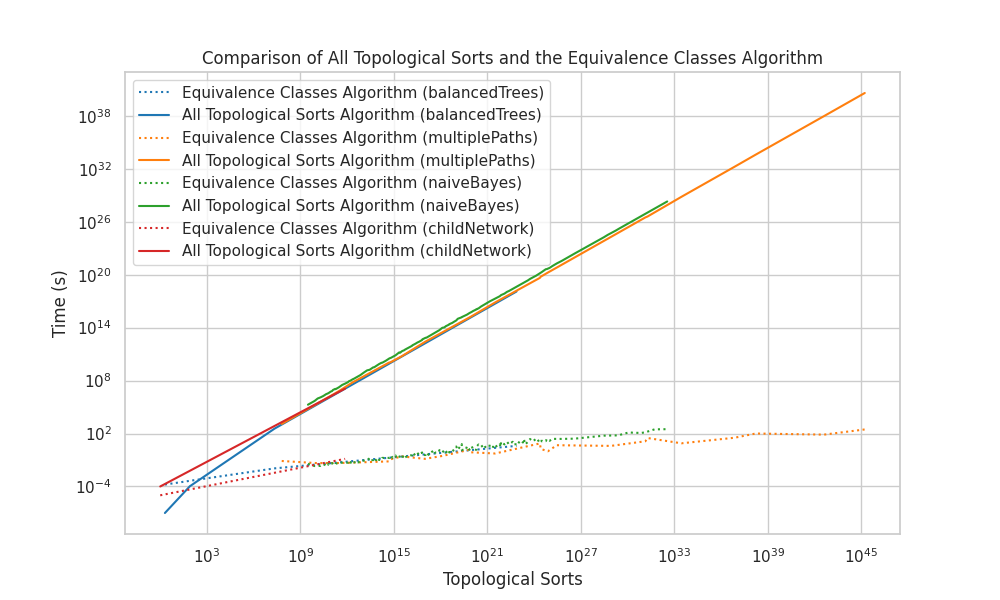
\includegraphics[width=\linewidth]{img/equivalentClassesVsAllToposorts_time.png}
		\caption{Runtime comparison between computing equivalence classes and enumerating all topological orders.\footnotemark}
		\label{fig:equivalenceClassesVsToposortsTimePlot}
	\end{subfigure}
	\hfill
	\begin{subfigure}[t]{0.48\linewidth}
		\vspace{0pt}
		\centering
		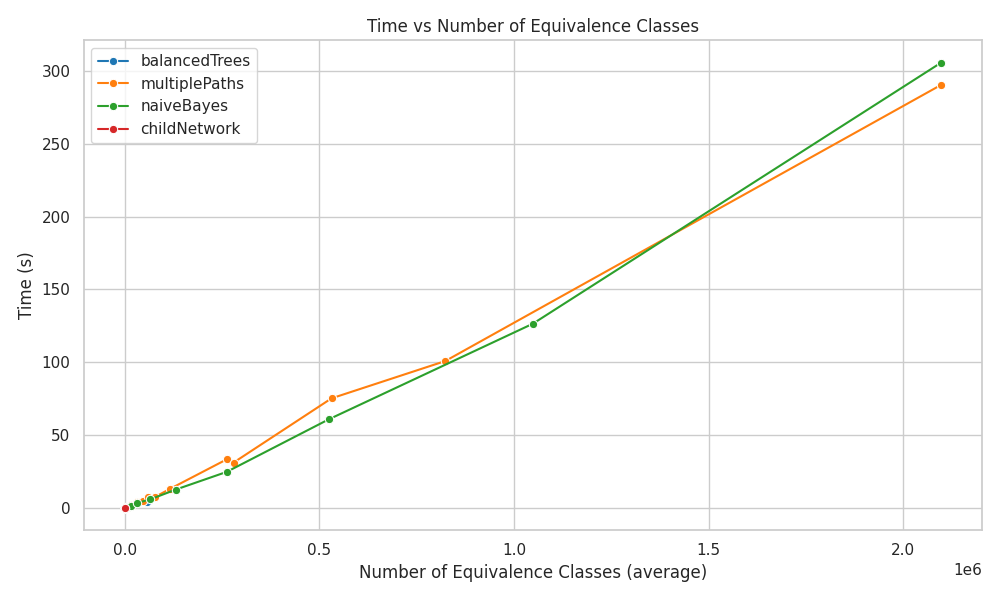
\includegraphics[width=\linewidth]{img/time_vs_equiv_classes.png}
		\caption{Runtime as a function of the number of equivalence classes.}
		\label{fig:timeVsEquivClasses}
	\end{subfigure}
	\label{fig:runtime_experiments}
\end{figure}
\footnotetext{To estimate runtime, we measured the time required to generate the first 1000 topological orders and extrapolated using the total number of orders in each graph, since full execution was not computationally feasible.}

Figure~\ref{fig:equivalenceClassesVsToposortsTimePlot} highlights the main advantage of our approach. While enumerating all topological orders quickly becomes infeasible (e.g., requiring days for large graphs), computing equivalence classes remains tractable.

\vspace{-3mm}

\paragraph{Sampling-Based Approximation of Topological Orders} We now evaluate the sampling-based approach.

\begin{figure}[H]
	\centering
	
	\begin{subfigure}[t]{0.32\linewidth}
		\vspace{0pt}
		\centering
		\small
		\setlength{\tabcolsep}{4pt}
		\renewcommand{\arraystretch}{1.1}
		\begin{tabular}{|r|r|}
			\hline
			\textbf{\# Samples} & \textbf{Time (s)}\\
			\hline
			100   & 0.9270 \\
			1000  & 1.1170 \\
			10000 & 4.7170 \\
			20000 & 7.7170 \\
			30000 & 10.8387 \\
			\hline
		\end{tabular}
		\caption{Sampling times for topological orders in \childNetwork{} using our developed algorithm.}
		\label{fig:samplingTimesTopoSorts}
	\end{subfigure}
	\hfill
	\begin{subfigure}[t]{0.64\linewidth}
		\vspace{0pt}
		\centering
		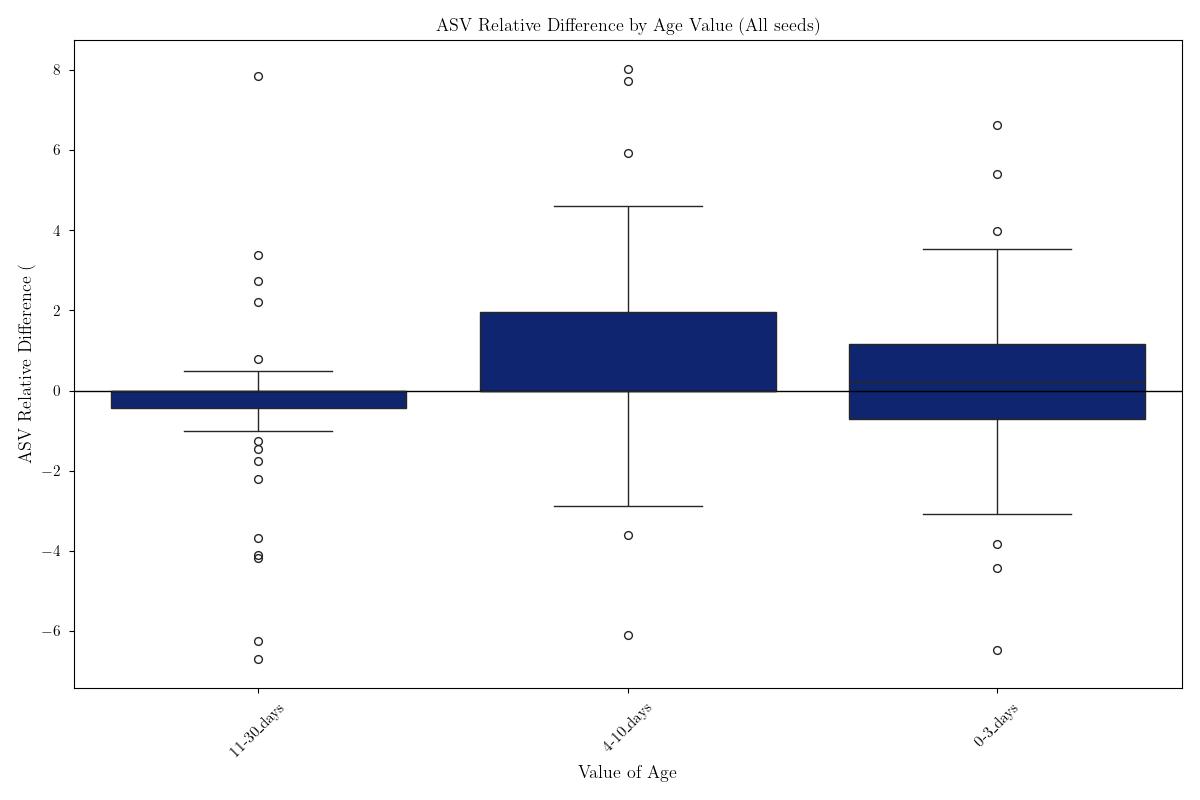
\includegraphics[width=0.80\linewidth]{img/ChildAllSeedsASVBoxplot.png}
		\caption{Relative error between approximate and exact ASV values in \childNetwork{}.}
		\label{fig:boxplotASVApproximateDifferences}
	\end{subfigure}
	\label{fig:sampling_results_combined}
\end{figure}

Table~\ref{fig:samplingTimesTopoSorts} shows that when using our algorithm the sampling remains efficient even for large numbers of samples. Moreover, the runtime is not linear in the number of samples, as multiple candidates are generated simultaneously during recursive calls due to our efficient implementation.
We conclude that in the bounded-degree setting (observe that in all the examples considered here most nodes have small degree) our algorithm is more efficient than the alternative options such as \cite{HUBER2006420}. Nevertheless, we recall that their algorithm is more general, as it applies beyond polytrees and runs in polynomial time.

Finally, we evaluate the approximation error of ASV using sampled orders. Figure~\ref{fig:boxplotASVApproximateDifferences} shows that using 1000 samples yields an average relative error of around $8\%$. Larger ASV values exhibit smaller relative error, while larger deviations correspond to very small true values.
These results indicate that sampling provides a practical trade-off between accuracy and computational cost.

\vspace{-3mm}

\paragraph{Remarks on Mean Prediction Computation} In our experiments, the cost of evaluating the characteristic function is not the dominant factor. This happens because for decision trees under Bayesian Network distributions with a polytree structure mean prediction can be computed exactly in an efficient way. In general models this might not be the case, but nonetheless due to Proposition~\ref{prop:sampling_to_compute_ASV} if sampling is used instead of exact computation the overall error of the approximation should not be extremely bad.

\section{Conclusions}



\begin{credits}

\subsubsection{\discintname}
for example: The authors have no competing interests to declare that are
relevant to the content of this article.
\end{credits}
%
% ---- Bibliography ----
%
\printbibliography

\end{document}